\chapter{Related Work}

\section{Machine Learning}
There are many classes problems that machine learning can be used to solve, such
as the following~\cite{introtoml}:

\begin{itemize}
  \item \textbf{Supervised Learning}: Predict a real valued output (regression)
    or select one of $C$ predefined categorical outputs (classification)
    for a given input vector. This also includes problems like anomaly detection,
    ranking, and regression.
  \item \textbf{Unsupervised Learning}: Find structure or regularity in a given
    set of input vectors. This includes problems like density estimation and 
    clustering
  \item \textbf{Reinforcement Learning}: Develop a policy that allows an agent
    to observe the state of its environment and take the actions that will 
    achieve a large cumulative reward in the long run~\cite{introtorl}.
\end{itemize}

ModelDB Server and Spark Client can store operations and models for supervised
and unsupervised learning problems. Reinforcement learning, however, is out
of scope for this thesis.

For a supervised learning problems, suppose there is a dataset $\mathcal{D}$ that
consists of $n$ pairs of $(\textbf{x}^{(i)}, y^{(i)})$. There is a
pair for each $i \in \{{1...n}\}$. The $\textbf{x}^{(i)}$ are $p$-dimensional feature
vecotrs the decribe the $i^{th}$ example. So, $x^{(i)} \in \mathbb{R}^{p}$. 
For classification, $y^{(i)}$ is the class associated with the $i^{th}$ example or
the regression target for that example. That is, $y^{(i)} \in \{1...C\}$ for classification
and $y^{(i)} \in \mathbb{R}$ for regression. The $\textbf{x}^{(i)}$ vectors
can also be expressed as a $n \times p$ matrix $\textbf{X}$.

A machine learning model is a function $f(\textbf{x}; \boldsymbol{\theta})$ where
$\boldsymbol{\theta}$ is a vector of model parameters (e.g. the weights of a linear regression
model or the encoded splits of a decision tree model). This function accepts an 
input vector $x \in \mathbb{R}^{p}$ and produces a real output (e.g. for regression)
or probability of being in a specific class (e.g. for classification).

When training a model, it is useful to split the dataset $\mathcal{D}$ into
a training set $\mathcal{D}_{train}$ and testing set $\mathcal{D}_{test}$. This ensures
that the model is evaluated on data it has not seen before. An objective function
$J(\boldsymbol{\theta}, \mathcal{D}_{train})$ is defined and $\boldsymbol{\theta}$ 
is chosen to maximize (or minimize, depending on the formulation) the objective function.

Machine learning also requires some hyperparameters (e.g. maximum depth of decision tree, regularization constant) 
to be set in order to guide the training of the model. One way to pick values for the hyperparameters
is to use a validation set. That is, the dataset $\mathcal{D}$ is broken into three pieces, 
$\mathcal{D}_{train}$, $\mathcal{D}_{validation}$, and $\mathcal{D}_{test}$. For each 
hyperparameter configuration, a model is trained on $\mathcal{D}_{train}$. Then, the model
is evaluated on $\mathcal{D}_{validation}$. Then, the chosen hyperparameter configuration
is the one that yielded the model that performed best on the validation set. 
Using a technique called cross validation can make better use of the data. In 
$k$-fold cross validation, $\mathcal{D}_{train}$ is broken into $k$ pieces (or folds) of roughly
equal size. Then, for a given hyperparameter configuration, a total of $k$ models are trained, each 
trained on all but one of the folds. Each model is evaluated on the fold that was left out,
and the resulting evaluation metrics are aggregated (e.g. averaged) to produce the evaluation
metric for the hyperparameter configuration. The hyperparameter configuration with the
largest evaluation metric is chosen as the best hyperparameter configuration. Then, a final
model is trained on the entire $\mathcal{D}_{train}$ and is then evaluated on $\mathcal{D}_{test}$ 
\cite{deeplearningbook}.

The above concepts are, of course, a tiny fraction of the concepts of machine learning. However,
they serve to inspire many of the abstraction in ModelDB Server and ModelDB Spark Client.

\section{Linear and Tree Models}
ModelDB Server and Spark Client have special support for Linear Regression, Logistic Regression, 
Decision Tree, Random Forest, and Gradient Boosted Tree models. Therefore, it is worth discussing
them briefly.

A linear regression model is a function $f(\textbf{x}; \boldsymbol{\theta}) = \boldsymbol{\theta}^{T}\textbf{x}$,
where $\boldsymbol{\theta} \in \mathbb{R}^{p}$. Requiring that all feature vectors have an first entry of 
1 allows the model to incorporate an intercept term.

A logistic regression model is not actually used for regression, it is used for 
binary ($C=2$) classification. Under appropriate assumptions, the logistic 
regression model aims to predict the likelihood that a given input feature vector
belongs to class 1. Concretely, the logistic regression function is: 
$f(\textbf{x}; \boldsymbol{\theta}) = \frac{\exp{\boldsymbol{\theta}^{T}\textbf{x}}}{1 + \exp{\boldsymbol{\theta}^{T}\textbf{x}}}$.
Its output lies between 0 and 1.

A decision tree model partitions the input space into non-overlapping regions, where all
points in the same region are assigned the same value. This value could be a class label
in the case of classification or a real value in the case of regression. For a given input vector,
the decision tree considers a different feature at each internal node. The input vector is forwarded
to a child node based on the value of the feature. This child node, if it is an internal node, then considers another
feature and performs the same process. Eventually, the input vector arrives at a leaf node. Each leaf node corresponds to
a region of the input space, and thus has an associated value (e.g. class label or real number), which is taken
to be the prediction for the input vector. An illustration of this is shown in Figure \ref{fig:sample_decision_tree}.

\begin{figure}
  \centering
  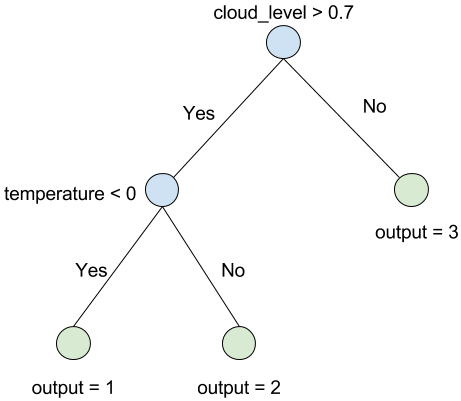
\includegraphics[height=3.0in]{sample_decision_tree}
  \caption{This is a decision tree model that could be used to predict whether the
  weather will be snowy (output 1), rainy (output 1), or neither (output 2) by
  looking at the cloud cover and temperature. The tree first checks if the cloud cover
  is high. If not, then it predicts there will be neither rain nor snow. Otherwise, the
  tree checks if the temperature is below 0. If so, then it predicts snow. Otherwise, it
  predicts rain.}
  \label{fig:sample_decision_tree}
\end{figure}

Random forest models and gradient boosted tree models are both ensembles of decision trees. They just differ in how they
are trained and applied. A random forest model trains many trees in parallel, where each tree is trained on a different bootstrapped
sample of the original dataset and where each split is only allowed to consider a subset of the features. A gradient boosted tree model
trains decision trees iteratively, where each successive decision tree learns to correct the mistakes of the previous trees. Like decision
trees, random forest and gradient boosted tree models can be used for both classification and regression. \cite{introtostatlearn}

\section{Spark ML}

\section{Machine Learning Libraries}

\section{Machine Learning Support Systems}
